\chapter{Data and Study Area}
\label{ch:data}

\section{Study Area}

The study area covers northern and central Germany with adjacent border regions
of the Czech Republic and Poland, bounded by longitudes $9.4^\circ$--$15.9^\circ$\,E
and latitudes $50.0^\circ$--$53.8^\circ$\,N.
This region spans approximately 430 km west to east and 440 km north to south,
encompassing the German federal states of Schleswig-Holstein, Hamburg, Bremen,
Mecklenburg-Vorpommern, Brandenburg, Berlin, Lower Saxony, Saxony-Anhalt, and
the northern parts of Saxony and Thuringia, as well as adjacent areas of
northern Bohemia (Czech Republic) and western Poland. The rectangular bounding
box intentionally extends beyond the German border to ensure adequate station
coverage for interpolation near boundary regions, avoiding edge effects that
would otherwise degrade prediction quality at the periphery of the domain.

The northern and central parts of the domain are dominated by the North German
Plain (\textit{Norddeutsche Tiefebene}), a broad lowland formed by
Pleistocene glaciation, with elevations predominantly below 200~m above sea
level.  The northern boundary meets the Baltic Sea coast, introducing maritime
influences on the precipitation regime.  Towards the south and southeast,
the terrain rises sharply: the Harz Mountains at the centre of the domain and
a continuous belt of uplands along the borders of southeastern Germany,
northern Bohemia, and southwestern Poland reach elevations above 1\,000~m;
these uplands include the Erzgebirge (Ore Mountains), the Thuringian Forest,
and the western Sudetes.

\textbf{Orographic lifting} \cite{daly1994prism} produces enhanced
precipitation on the windward (north-western) slopes of the southern
mountain ranges, while the lee sides and interior basins receive
substantially less, a phenomenon known as the \textbf{rain shadow} effect.
As a result, annual precipitation totals range from roughly
500--600~mm on the sheltered lowlands to over 1\,000~mm in the highest
parts of the Harz and the Erzgebirge, as computed from the ReKIS station
network (Table~\ref{tab:elevation_means}).
This large-scale orographic gradient makes the region a challenging
testbed for spatial interpolation methods.

All spatial computations use the ETRS89-LAEA coordinate reference system
(EPSG:3035), an equal-area projection appropriate for European studies, ensuring
that areas are preserved accurately across the domain, with distance
distortion remaining below 1\% at this regional scale.
The primary prediction target is a regular 1~km $\times$ 1~km grid
containing 189{,}648 cells; the best-performing method is additionally
applied at coarser spatial resolutions.
Table~\ref{tab:terrain-zones} shows how these cells are distributed across
three elevation zones: about 71\% of the domain lies on the lowland plain,
while about 7.5\% falls in mountainous terrain above 500~m.

\begin{table}[ht]
  \centering
  \caption{Distribution of the 1~km prediction grid cells across terrain zones}
  \label{tab:terrain-zones}
  \begin{tabular}{lccc}
    \toprule
    Terrain zone & Elevation range & Grid cells & Share \\
    \midrule
    Plains    & 0--250~m   & 133{,}970 & 70.6\% \\
    Hills     & 250--500~m &  41{,}411 & 21.8\% \\
    Mountains & $>$500~m   &  14{,}267 &  7.5\% \\
    \bottomrule
  \end{tabular}
\end{table}

\section{Observational Data: ReKIS Station Network}

\subsection{Network Description}

Daily precipitation measurements were obtained from the Regionales
Klimainformationssystem (ReKIS), a regional climate information system
providing quality-controlled station data for northern and central Germany.%
\footnote{ReKIS is operated by the Saxon State Office for the
Environment, Agriculture and Geology (LfULG); see
\url{https://www.rekis.org}.}
The dataset covers 2{,}458 stations with continuous daily records spanning the
full analysis period from January~1,~1961 -- December~31,~2023, yielding
63 years of daily precipitation observations (Figure~\ref{fig:station}).
All stations report at least one wet day in every year of the record, indicating
uniform temporal coverage across the network with no station dropouts or
gaps in network density over time.
This long, spatially consistent record supports reliable estimation of
climatological monthly precipitation normals, which are used as a detrending
baseline in the interpolation pipeline (Section~\ref{sec:detrending}).

\begin{figure}[htbp]
    \centering
    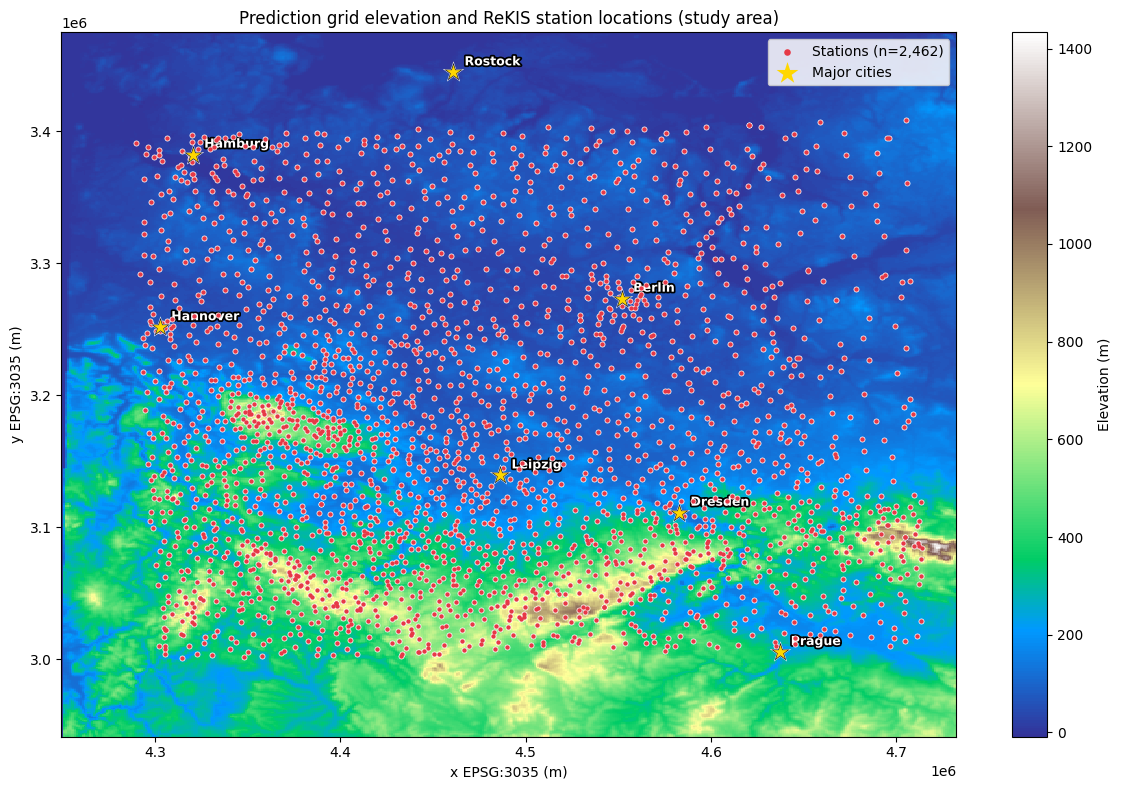
\includegraphics[width=0.95\textwidth]{images/03/station.png}
    \caption{The 2{,}458 ReKIS stations used in this study}
    \label{fig:station}
\end{figure}

\subsection{Quality Control}

A systematic quality control check was applied to the raw ReKIS data prior
to analysis.
Across all 56{,}650{,}620 station-day records, \textbf{no missing values and no
negative precipitation amounts} were detected, confirming the high completeness
of the network.

Two issues were identified and corrected.
First, 38 station IDs (predominantly cross-border Czech and Polish gauges)
appeared two or three times in the metadata catalogue with identical coordinates;
duplicates were removed, keeping one entry per station ID.
Second, four pairs of stations with distinct IDs shared identical geographic
coordinates, representing co-located gauges that would cause rank deficiency
in the kriging covariance matrix; these were merged by averaging their daily
records.
Together these corrections reduce the network from 2{,}462 to 2{,}458 unique
station locations.

\newpage
\section{Auxiliary Data}

\subsection{Digital Elevation Model}

\noindent\begin{minipage}[t]{0.50\textwidth}
\vspace{0pt}
Terrain elevation data were derived from the Copernicus Digital Elevation Model
\cite{copernicus_dem}, resampled to the same 1 km $\times$ 1 km grid as the
prediction target (Figure~\ref{fig:elevation}).
Elevation is used as a covariate when interpolating monthly precipitation
normals (the long-term mean monthly totals from the 1961--2023 station
record). Under the 3D thin-plate spline variant, these normals are
interpolated as a function of $(x, y, z_\text{elev})$, where $x$ and $y$
are the EPSG:3035 projected coordinates and $z_\text{elev}$ is terrain
elevation from the Copernicus DEM, rather than spatial coordinates alone.
This lets the model capture orographic enhancement of precipitation.
\end{minipage}
\hfill
\begin{minipage}[t]{0.47\textwidth}
\vspace{0pt}
\centering
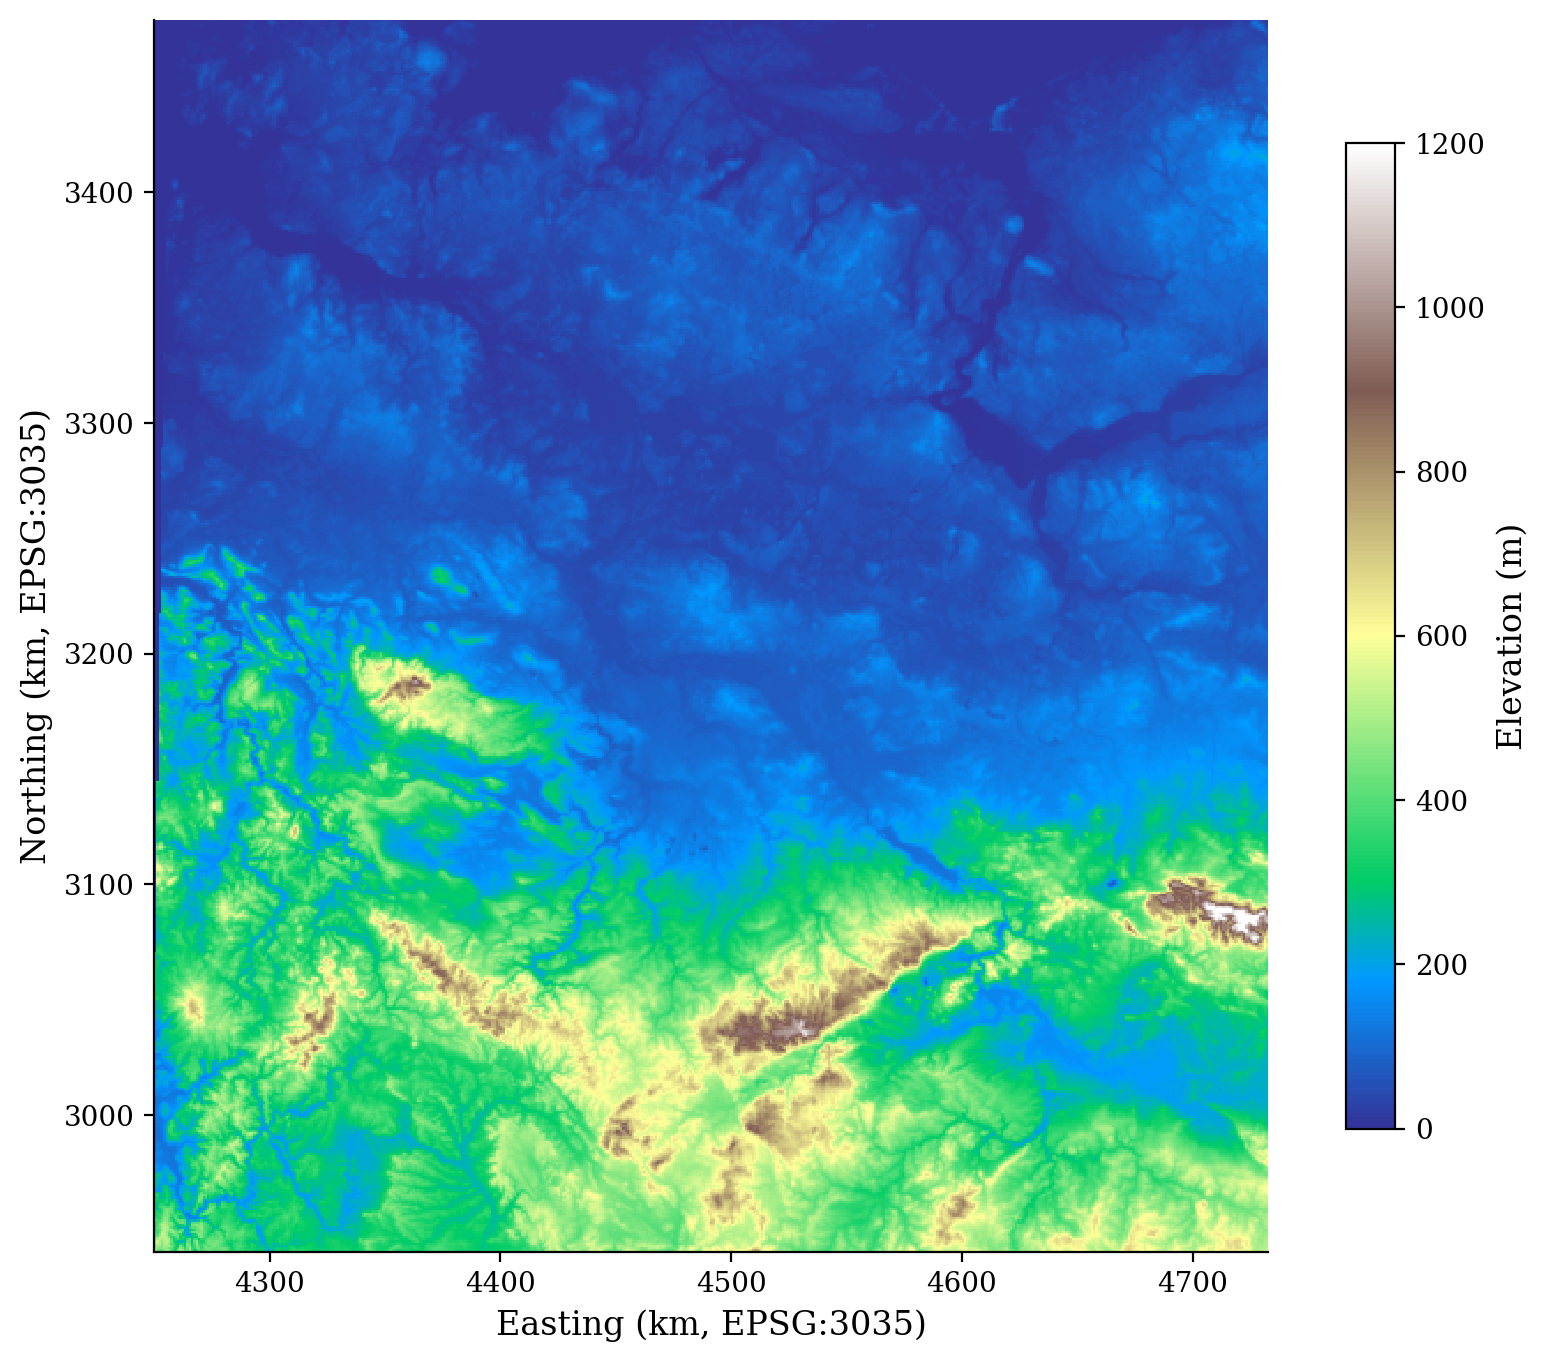
\includegraphics[width=\linewidth]{images/03/elevation.png}
\captionof{figure}{Elevation over the study area (Copernicus DEM, resampled to the 1~km grid)}
\label{fig:elevation}
\end{minipage}

\subsection{SoilGrids Auxiliary Variables}

\noindent\begin{minipage}{\textwidth}
Six soil properties from SoilGrids \cite{poggio2021soilgrids} are used
as auxiliary covariates for the gradient boosting model (LightGBM) and
the Bayes Neural Field: bulk density, clay content, sand content, silt
content, soil organic carbon, and volumetric water content at $-10$~kPa.
Each variable is averaged across the 0--30~cm depth range, yielding one
value per grid cell (Figure~\ref{fig:soilgrids}).

\vspace{0.8em}
\centering
\includegraphics[width=0.95\textwidth]{images/03/fig_soilgrids.png}
\captionof{figure}{SoilGrids auxiliary variables over the study area}
\label{fig:soilgrids}
\end{minipage}

\section{Statistical Properties of Daily Precipitation}
\label{sec:precip_statistics}

Daily precipitation data have several statistical properties that
directly complicate interpolation.
These properties drive the preprocessing and modelling choices
described in subsequent chapters.

\subsection{Zero-Inflation and Mixed Distribution}

Daily precipitation is intermittent: on any given day, a large fraction of
stations record no precipitation (dry days), while the remaining stations record
positive amounts.
This yields a mixed discrete-continuous distribution, a point mass at zero
combined with a right-skewed continuous component for positive values.
The proportion of dry days varies by season and location but typically exceeds
50\,\% across the study area \cite{haylock2008european}
(Figure~\ref{fig:precip_distribution}).

Standard interpolation methods designed for continuous Gaussian fields cannot
handle this mixed distribution.
The two-stage model described in Chapter~\ref{ch:kriging} addresses this
directly: a binary indicator stage separates wet from dry locations, and a
separate amount model is applied only to wet-day observations.

\begin{figure}[H]
    \centering
    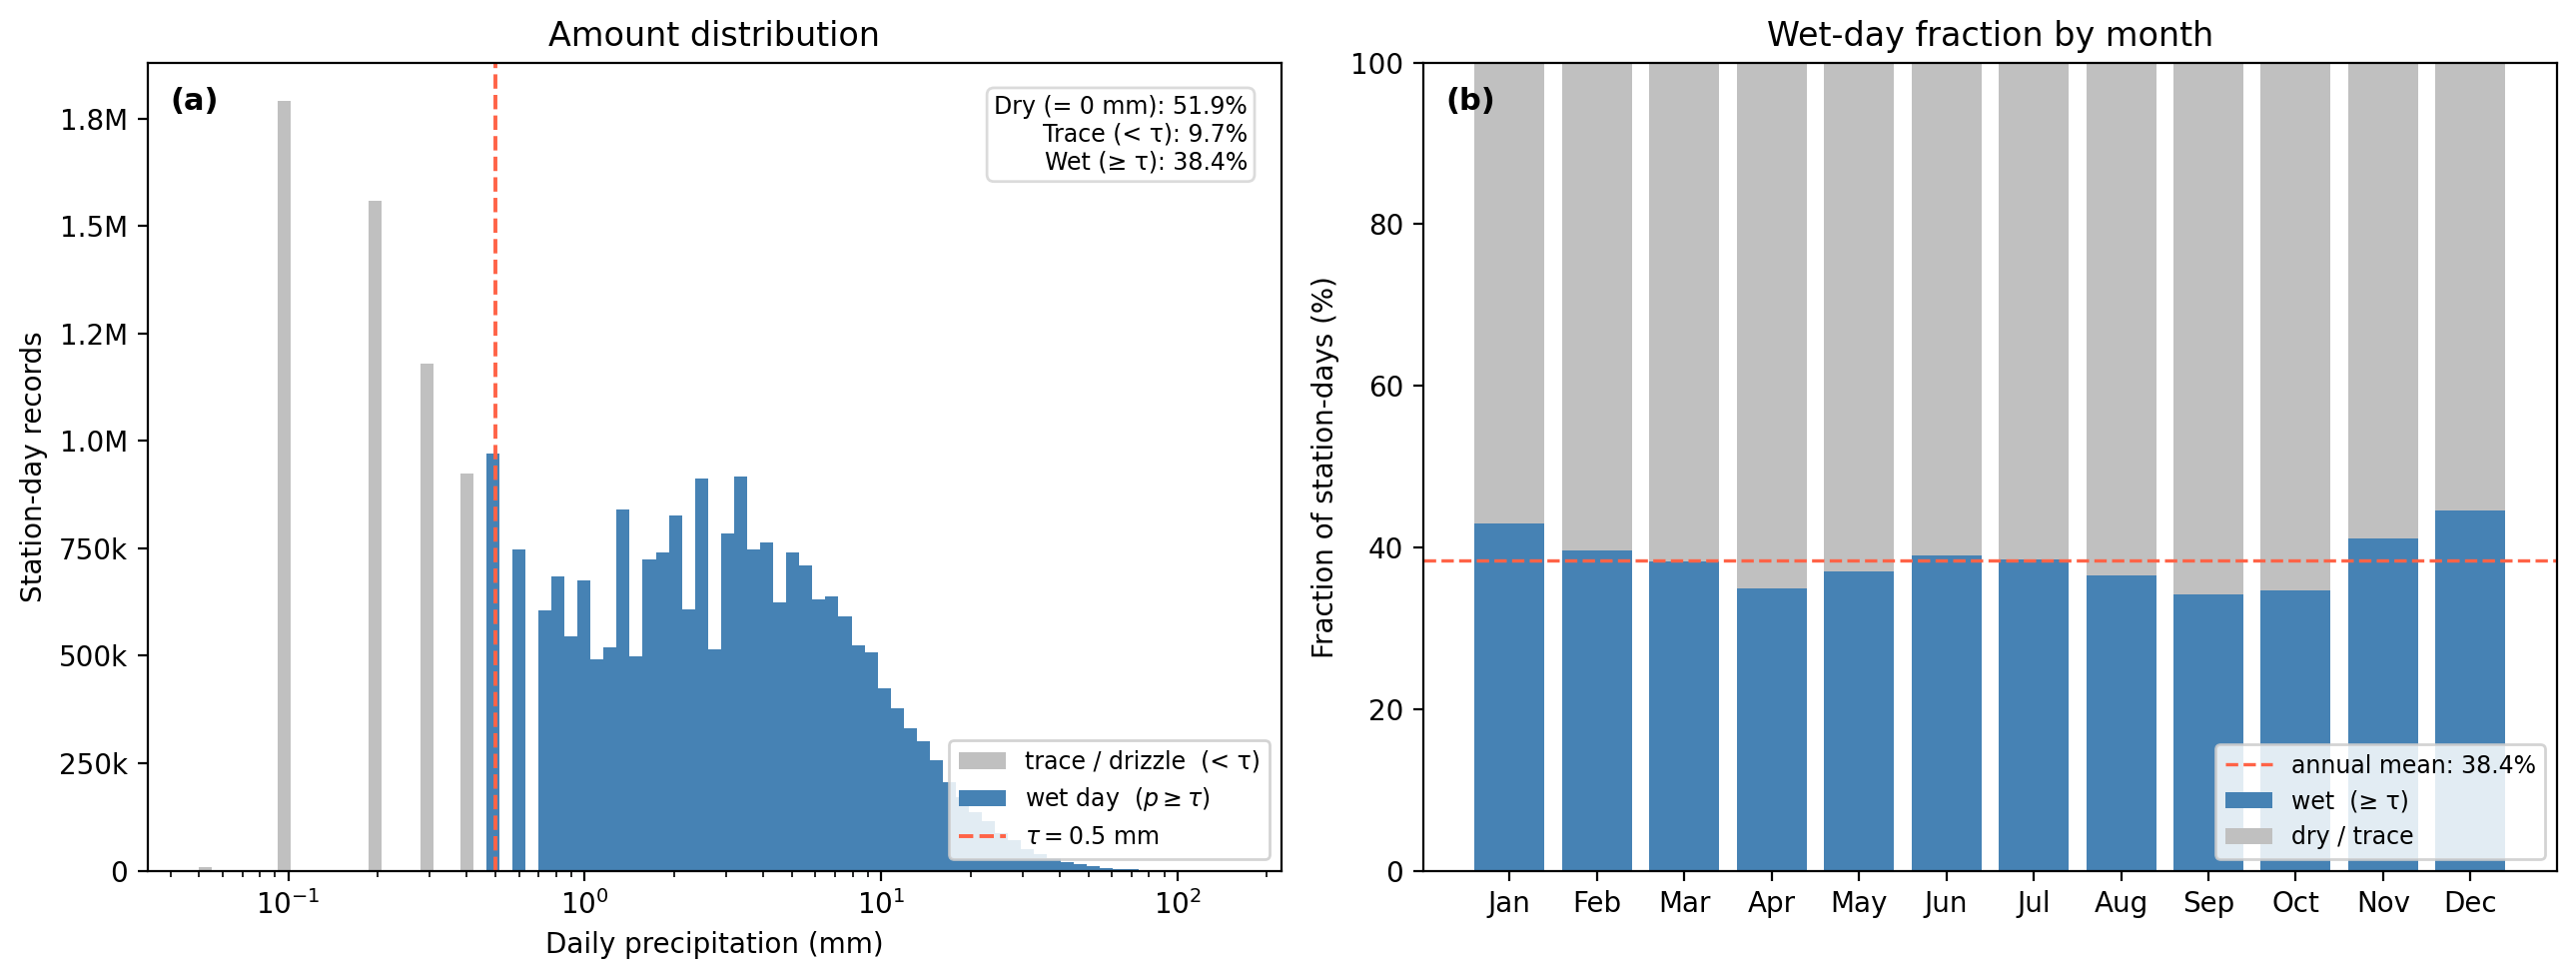
\includegraphics[width=0.95\textwidth]{images/03/fig_precip_distribution.png}
    \caption{Mixed discrete-continuous distribution of daily precipitation
    in the ReKIS network (1961--2023). Panel~(a): histogram of non-zero
    amounts on a log scale; dry-day fraction (51.9\,\%) and the wet-day
    threshold $\tau = 0.5$~mm are marked. Panel~(b): wet-day fraction
    by calendar month}
    \label{fig:precip_distribution}
\end{figure}

\subsection{Right-Skewed Amounts}

When conditioned on wet days, precipitation amounts follow a heavily
right-skewed distribution.
Rare but intense rainfall events contribute disproportionately to total
accumulation, producing a long upper tail \cite{hofstra2008comparison}
(Figure~\ref{fig:wetday_skewness}).
Climatological normalisation is applied before kriging to remove seasonal
non-stationarity and stabilise variance (Section~\ref{sec:detrending}).

\begin{figure}[H]
    \centering
    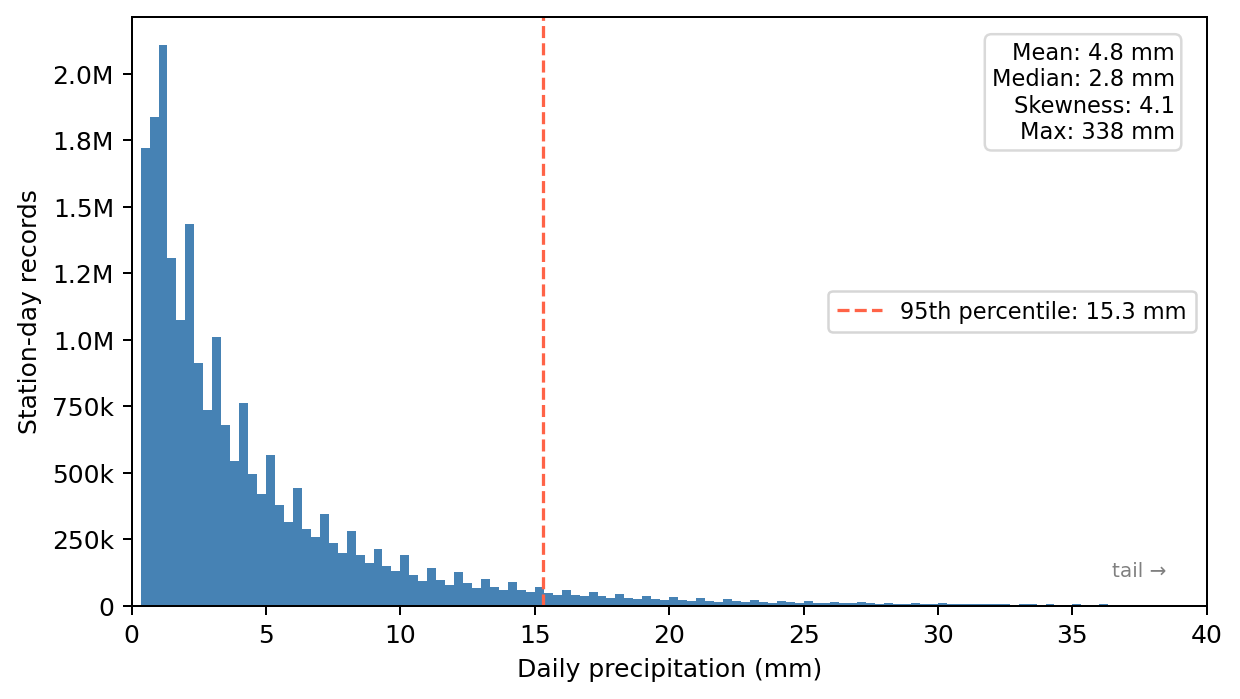
\includegraphics[width=0.7\textwidth]{images/03/fig_wetday_skewness.png}
    \caption{Distribution of wet-day precipitation amounts ($p \geq 0.5$~mm)
    across all ReKIS stations (1961--2023). The mean (4.8~mm) exceeds the
    median (2.8~mm) and the skewness is 4.1, confirming the heavy right tail.
    The 95th percentile (15.3~mm) is marked; extreme values extend to
    338~mm}
    \label{fig:wetday_skewness}
\end{figure}

\subsection{Seasonality and Non-Stationarity}

Precipitation in northern Germany shows strong seasonal variation.
Monthly mean values at the observational stations range from approximately 43.5~mm in
February to 74.7~mm in July (Figure~\ref{fig:monthly_means}).
This seasonal cycle is a large-scale non-stationarity that violates
the stationarity assumption of ordinary kriging.
Climatological normalisation in Chapter~\ref{ch:kriging} (Section~\ref{sec:detrending})
addresses it.

\begin{figure}[H]
    \centering
    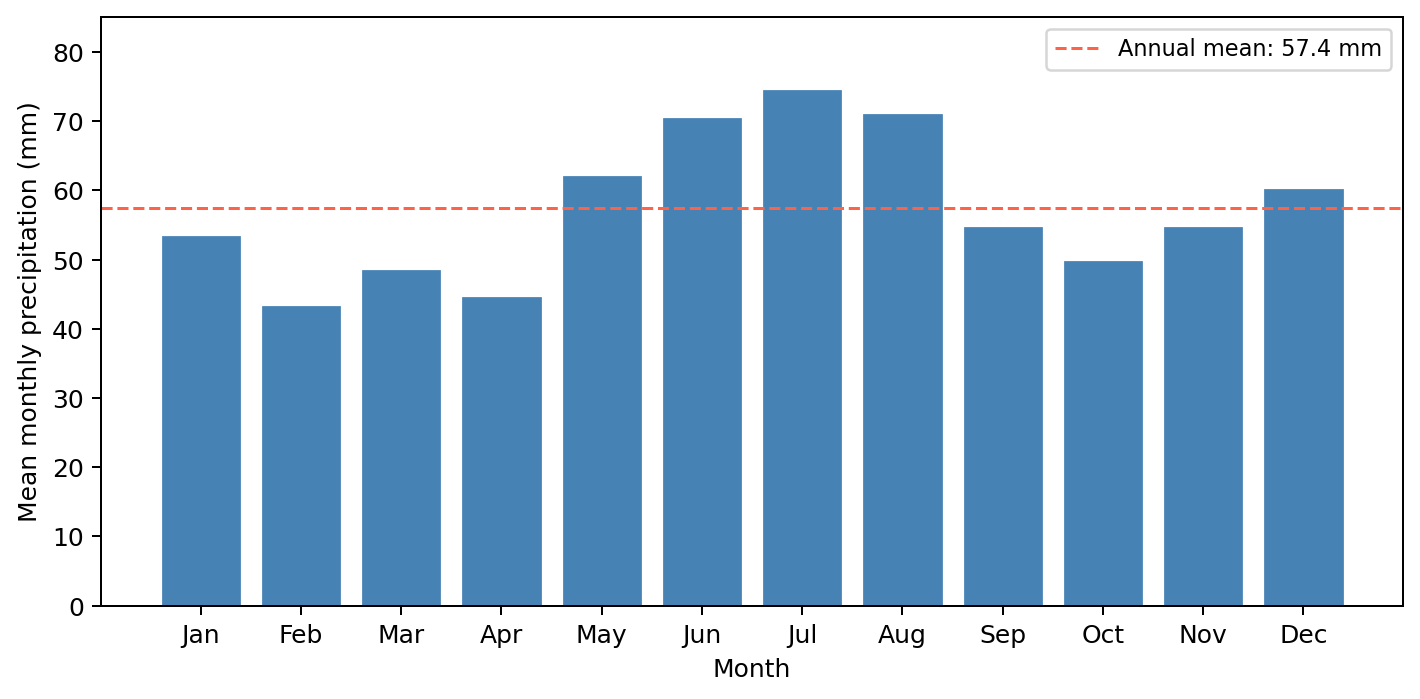
\includegraphics[width=0.8\textwidth]{images/03/fig_monthly_means.png}
    \caption{Mean monthly precipitation averaged over all ReKIS stations
    (1961--2023). The dashed line marks the annual mean of 57.4~mm}
    \label{fig:monthly_means}
\end{figure}

\subsection{Orographic Effects}

\begin{sloppypar}
Terrain elevation strongly affects precipitation, particularly
during winter months when frontal systems interact with topography
\cite{daly1994prism}.
In the study area, mean monthly precipitation at stations in the mountainous zone
(above 500~m) is approximately 85.9~mm, compared to 50.7~mm in the plains
(Table~\ref{tab:elevation_means}).
This orographic gradient reflects frontal systems interacting with
the mountainous terrain along the southern part of the domain.
\end{sloppypar}

\begin{table}[ht]
\centering
\caption{Mean monthly precipitation by terrain elevation zone (ReKIS, 1961--2023)}
\label{tab:elevation_means}
\begin{tabular}{lrrr}
\toprule
Elevation zone & N stations & Mean elev. (m) & Mean precip. (mm) \\
\midrule
Plains (0--250 m)    & 1{,}530 & 101 & 50.7 \\
Hills (250--500 m)   &    667  & 352 & 61.5 \\
Mountains (500+ m)   &    265  & 661 & 85.9 \\
\bottomrule
\end{tabular}
\end{table}
